\subsection{Drawer}\label{sec:launcher:drawer}
The drawer is a separate view that is situated on the left-hand side of \homeactivity.
Its main purpose is to allow \launcher users to apply a new colour scheme to the installed \giraf applications.

To avoid cluttering the screen, the drawer can be shown and hidden at will.
This means that the only part of the drawer that is visible at all times is the sidebar, which can be dragged towards the centre of the screen to reveal the content of the drawer.
The sidebar also contains the informative widgets described in \cref{sec:launcher}.

Illustrations of the drawer in closed and opened state can be seen in \cref{fig:drawerclosed,fig:draweropened} respectively.

\begin{figure}[h] % Billeder af draweren i åben og lukket tilstand
\centering
	\begin{subfigure}[b]{.48\textwidth}
	\centering
	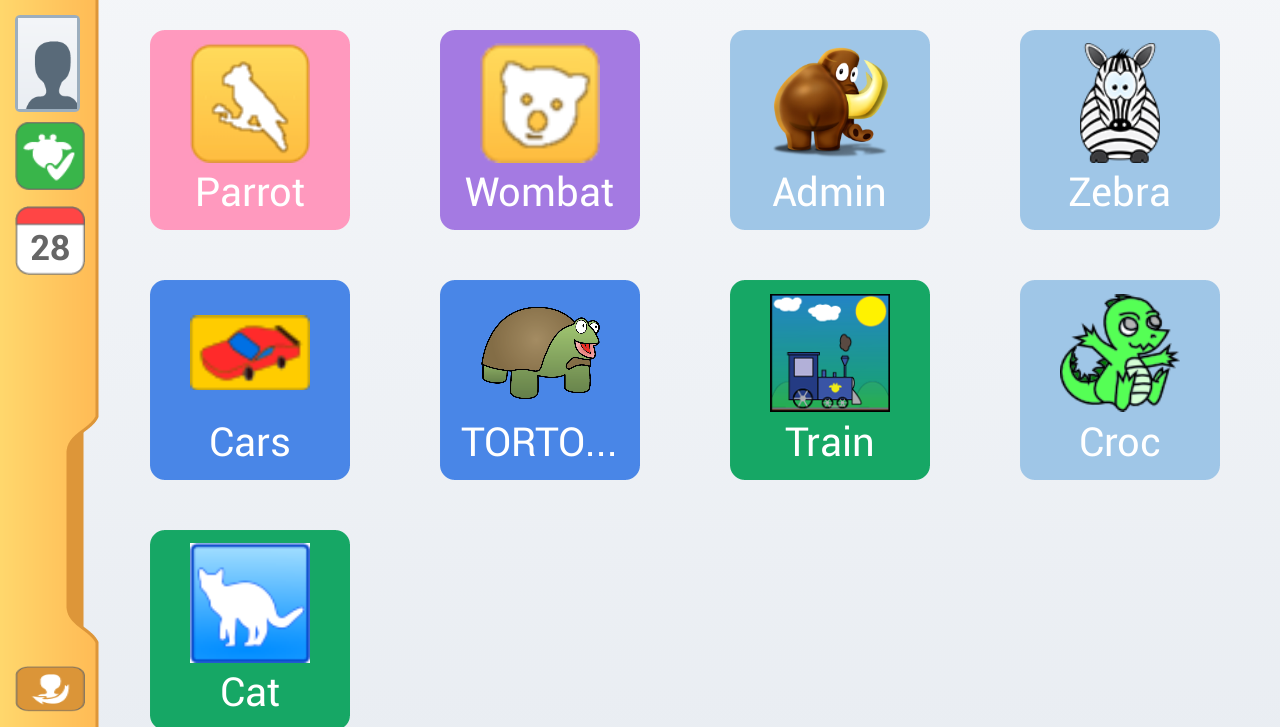
\includegraphics[width=\textwidth]{screenshots-old-giraf/giraf-homeactivity.png}
	\caption{Drawer closed.}
	\label{fig:drawerclosed}
	\end{subfigure}
	\hfill
	\begin{subfigure}[b]{.48\textwidth}
	\centering
	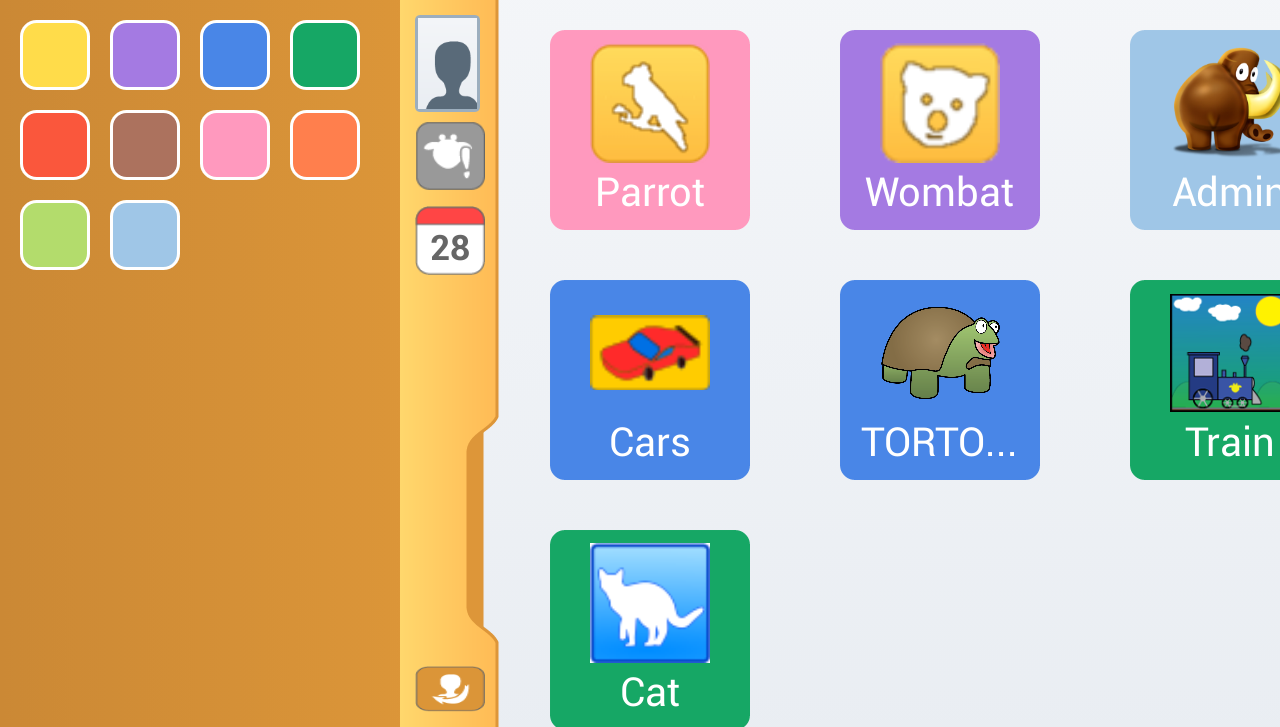
\includegraphics[width=\textwidth]{screenshots-old-giraf/giraf-drawer-fullyextended.png}
	\caption{Drawer fully opened.}
	\label{fig:draweropened}
	\end{subfigure}
\caption{States of the drawer component shown in \homeactivity.}
\label{fig:drawerstates}
\end{figure}

As indicated by \cref{fig:drawerstates}, the drawer already meet the requirement that a colour can be dragged onto an application.
In spite of this, many deficiencies have been located, which are further enlightened by the following sections.

\subsubsection{Behaviour of the Drawer}\label{sec:drawer:behaviour}
The drawer opens by dragging the sidebar to the right.
While being opened, the drawer pushes the application icons along with it to the right, resulting in some icons disappearing out of view.
Furthermore, the drawer stops sliding when pressure is released from the touch-screen, meaning it can be left in a half-open, half-closed state.
To change the colour of an application, a colour can be dragged and dropped onto an application icon. 
The result is immediately apparent, as the colour framing the icon changes to the selected colour.

\subsubsection{Desired Improvements}
Since no formal requirements are available and we have not yet held a meeting with the clients, the suggested improvements below is based on what we find to be natural requirements of such an user interface component. 

\begin{itemize}
\item The drawer should be either open or closed. 
A half-open or half-closed state should result in the drawer popping into the state closest to its current position.
\item The drawer should close while a colour is being dragged, and open again when the colour is dropped.
\item The drawer should not push the application icons out of the screen.
\item The source code responsible for the animation of the drawer and the layout of \homeactivity should be refactored in order to
	\begin{itemize}
	\item take advantage of standard Android animations and layout features,
	\item allow the activity to dynamically adjust according to display-size and
	\item reduce the amount of clutter in and improve readability of the source code .
	\end{itemize}
\end{itemize}

The implementation of the improvements is described in \cref{sec:developments:drawerimprovements}.